%%%% proposta_pt.tex
%%%% Project specification paper based on the IJCAI--ECAI 26 template.
%%%% Base: latex/proposta_IAHC_DINIS_ROSA.pdf (texto original).
%%%% Cores: apenas vermelho mantido, por indicação do utilizador.

\typeout{Project paper using IJCAI--ECAI 26 formatting}

\documentclass{article}
\pdfpagewidth=8.5in
\pdfpageheight=11in

% Official IJCAI--ECAI 26 style file.
% Compile from the latex/ directory so the relative path resolves correctly.
\usepackage{FormattingGuidelines-IJCAI-ECAI-26/ijcai26}

% Packages required/recommended by the official template.
\usepackage{times}
\usepackage{soul}
\usepackage{url}
\usepackage[hidelinks]{hyperref}
\usepackage[utf8]{inputenc}
\usepackage[small]{caption}
\usepackage{graphicx}
\usepackage{tikz}
\usetikzlibrary{positioning,arrows.meta}
\usepackage{amsmath}
\usepackage{amsthm}
\usepackage{booktabs}
\usepackage{algorithm}
\usepackage{algorithmic}
% REV-013 — cor #808000, RGB (128, 128, 0) (mesma do REVISION_LOG.md). Texto movido para REV-018.
% REV-018 — cor #5C6BC0, RGB (92, 107, 192) (mesma do REVISION_LOG.md). Macro \revtext para as revisões coloridas.
% REV-020 — cor #607D8B, RGB (96, 125, 139) (mesma do REVISION_LOG.md).
% REV-021 — cor #D500F9, RGB (213, 0, 249) (mesma do REVISION_LOG.md).
% REV-022 — cor #00897B, RGB (0, 137, 123) (mesma do REVISION_LOG.md).
% REV-023 — cor #0277BD, RGB (2, 119, 189) (mesma do REVISION_LOG.md). Títulos de subsecções novos.
% REV-042 — cor #0A3D62, RGB (10, 61, 98) (mesma do REVISION_LOG.md). HMM e Wu et al. deixam de ser comparações (resumo, objetivos, avaliação, pós-processamento).
% REV-041 — cor #FF1744, RGB (255, 23, 68) (mesma do REVISION_LOG.md). Baseline fechada; CNN de referência única (secções 4 e 5) e secção de Resultados.
% REV-040 — cor #7F0000, RGB (127, 0, 0) (mesma do REVISION_LOG.md). Baseline congelada: treino de 300 épocas, seleção no teste e resultados regenerados por código.
% REV-036 — cor #00C853, RGB (0, 200, 83) (mesma do REVISION_LOG.md). Papéis dos conjuntos reservados: teste seleciona, validação mede no fim.
% REV-035 — cor #6200EA, RGB (98, 0, 234) (mesma do REVISION_LOG.md). Resultados do treino final, números gerados por código.
% REV-032 — cor #D81B60, RGB (216, 27, 96) (mesma do REVISION_LOG.md). Primeira execução de treino.
% REV-031 — cor #006064, RGB (0, 96, 100) (mesma do REVISION_LOG.md). Anexo com as figuras do ensaio preliminar.
% REV-030 — cor #FF6F00, RGB (255, 111, 0) (mesma do REVISION_LOG.md). Subsecção e figuras do ensaio preliminar (marcador de resultados).
% REV-028 — cor #00ACC1, RGB (0, 172, 193) (mesma do REVISION_LOG.md). Avaliação em 3 outras viagens de treino.
% REV-027 — cor #AFB42B, RGB (175, 180, 43) (mesma do REVISION_LOG.md). Ensaio de ajuste em 3 viagens de treino.
% REV-026 — cor #2E7D32, RGB (46, 125, 50) (mesma do REVISION_LOG.md). Figura do desenho da CNN 1D.
% REV-025 — cor #6A1B9A, RGB (106, 27, 154) (mesma do REVISION_LOG.md). Secção «Especificação da CNN 1D de referência».
% REV-024 — cor #6D4C41, RGB (109, 76, 65) (mesma do REVISION_LOG.md). Implementação do Marco 3 (sequências, normalização, CNN, testes).
\definecolor{rev013}{RGB}{128,128,0}
\definecolor{rev018}{RGB}{92,107,192}
\definecolor{rev020}{RGB}{96,125,139}
\definecolor{rev021}{RGB}{213,0,249}
\definecolor{rev022}{RGB}{0,137,123}
\definecolor{rev023}{RGB}{2,119,189}
\definecolor{rev024}{RGB}{109,76,65}
\definecolor{rev025}{RGB}{106,27,154}
\definecolor{rev026}{RGB}{46,125,50}
\definecolor{rev027}{RGB}{175,180,43}
\definecolor{rev028}{RGB}{0,172,193}
\definecolor{rev030}{RGB}{255,111,0}
\definecolor{rev031}{RGB}{0,96,100}
\definecolor{rev032}{RGB}{216,27,96}
\definecolor{rev035}{RGB}{98,0,234}
\definecolor{rev036}{RGB}{0,200,83}
\definecolor{rev040}{RGB}{127,0,0}
\definecolor{rev041}{RGB}{255,23,68}
\definecolor{rev042}{RGB}{10,61,98}
\newcommand{\revtext}[2]{{\color{#1}#2}}
% Números gerados por ais.cli.build_final_results (REV-035): \rv{\resXxx} mostra o valor na cor da revisão.
% Gerado por ais.cli.build_final_results em 2026-11-24T00:35:51+00:00 (commit 9ab2e46cf).
% NÃO EDITAR À MÃO: volta a gerar-se a partir de results/baseline_frozen/final_results.json.
\newcommand{\resDadosLinhas}{1\,026\,279}
\newcommand{\resDadosViagens}{123}
\newcommand{\resDadosLinhasTreino}{713\,854}
\newcommand{\resDadosViagensTreino}{87}
\newcommand{\resDadosPercPesca}{75,4\,\%}
\newcommand{\resPrepCoincide}{99,9997\,\%}
\newcommand{\resPrepBearingMediana}{1,1}
\newcommand{\resModParametros}{21\,761}
\newcommand{\resModCampo}{13}
\newcommand{\resModParamA}{1\,152}
\newcommand{\resModParamB}{10\,304}
\newcommand{\resModParamC}{10\,272}
\newcommand{\resModParamD}{33}
\newcommand{\resTrViagens}{87}
\newcommand{\resTrPontos}{713\,854}
\newcommand{\resTrEpocas}{300}
\newcommand{\resTrMaxEpocas}{300}
\newcommand{\resTrSegundos}{19}
\newcommand{\resTrSegPorEpoca}{2,8}
\newcommand{\resTrOrcamentoMin}{25}
\newcommand{\resTrSemente}{42}
\newcommand{\resTrTorch}{2.15.0}
\newcommand{\resSelEpoca}{162}
\newcommand{\resSelLimiar}{0,65}
\newcommand{\resSelNCand}{300}
\newcommand{\resSelViagens}{18}
\newcommand{\resSelPontos}{103\,409}
\newcommand{\resSelPerdaTeste}{0,185}
\newcommand{\resSelPerdaTesteMax}{0,342}
\newcommand{\resSelPerdaTreino}{0,149}
\newcommand{\resSelGrelhaMin}{0,05}
\newcommand{\resSelGrelhaMax}{0,95}
\newcommand{\resTreinoPontos}{713\,854}
\newcommand{\resTreinoErros}{46\,312}
\newcommand{\resTreinoAcc}{93,5\,\%}
\newcommand{\resTreinoAccMaj}{75,4\,\%}
\newcommand{\resTreinoPercPesca}{75,4\,\%}
\newcommand{\resTreinoNavReal}{175\,584}
\newcommand{\resTreinoPescaReal}{538\,270}
\newcommand{\resTreinoNavPrec}{0,832}
\newcommand{\resTreinoNavSens}{0,923}
\newcommand{\resTreinoNavF}{0,875}
\newcommand{\resTreinoNavIoU}{0,778}
\newcommand{\resTreinoPescaPrec}{0,974}
\newcommand{\resTreinoPescaSens}{0,939}
\newcommand{\resTreinoPescaF}{0,956}
\newcommand{\resTreinoPescaIoU}{0,916}
\newcommand{\resTreinoTN}{162\,072}
\newcommand{\resTreinoFP}{13\,512}
\newcommand{\resTreinoFN}{32\,800}
\newcommand{\resTreinoTP}{505\,470}
\newcommand{\resTestePontos}{103\,409}
\newcommand{\resTesteErros}{5\,502}
\newcommand{\resTesteAcc}{94,7\,\%}
\newcommand{\resTesteAccMaj}{61,2\,\%}
\newcommand{\resTestePercPesca}{61,2\,\%}
\newcommand{\resTesteNavReal}{40\,122}
\newcommand{\resTestePescaReal}{63\,287}
\newcommand{\resTesteNavPrec}{0,900}
\newcommand{\resTesteNavSens}{0,971}
\newcommand{\resTesteNavF}{0,934}
\newcommand{\resTesteNavIoU}{0,876}
\newcommand{\resTestePescaPrec}{0,981}
\newcommand{\resTestePescaSens}{0,931}
\newcommand{\resTestePescaF}{0,955}
\newcommand{\resTestePescaIoU}{0,915}
\newcommand{\resTesteTN}{38\,964}
\newcommand{\resTesteFP}{1\,158}
\newcommand{\resTesteFN}{4\,344}
\newcommand{\resTesteTP}{58\,943}
\newcommand{\resTesteViagMin}{74,0\,\%}
\newcommand{\resTesteViagMed}{97,1\,\%}
\newcommand{\resTesteViagMax}{99,8\,\%}
\newcommand{\resTestePiorViagem}{\texttt{220006000-2}}
\newcommand{\resTesteNViagNaoSuperam}{0}

\newcommand{\rv}[1]{#1}
\usepackage[switch]{lineno}

% Keep line numbers enabled for a submission. Disable for camera-ready.
\linenumbers
\switchlinenumbers

\urlstyle{same}

% Optional theorem environments.
\newtheorem{example}{Example}
\newtheorem{theorem}{Theorem}

% Required PDF metadata block. Keep unchanged.
\pdfinfo{
/TemplateVersion (IJCAI.2026.0)
}

\title{OOI  Segmenta\c{c}\~ao sem\^antica de trajet\'orias AIS para dete\c{c}\~ao de atividade de pesca usando janelas sobrepostas e p\'os-processamento temporal}

% For an anonymous submission, replace this block with the track-approved
% anonymous author declaration. For the camera-ready version, provide all
% author and affiliation information.
\author{
    Dinis Soveral Botelho Rosa
    \affiliations
    University of Coimbra / Department of Informatics Engineering
    \emails
    dinisrosa22@gmail.com
}

\begin{document}

\maketitle

\begin{abstract}
A pesca ilegal, não declarada e não regulamentada (IUU) ameaça a sustentabilidade dos oceanos. O \emph{Automatic Identification System} (AIS) permite monitorizar navios à escala global, mas converter trajetórias em deteções úteis à fiscalização exige métodos robustos e interpretáveis. Propõe-se investigar se a combinação de janelas sobrepostas e pós-processamento temporal melhora a qualidade e a estabilidade da segmentação semântica de trajetórias AIS para detetar pesca, como apoio à decisão de inspetores humanos (\textcolor{red}{\emph{human-on-the-loop}}), segundo princípios de Inteligência Artificial Centrada no Humano (HCAI): explicabilidade, confiança calibrada e decisão humana final. A avaliação usa \rv{\resDadosViagens} trajetórias anotadas (Kaggle), \revtext{rev042}{comparando a CNN sobre a viagem completa com a CNN sobre janelas sobrepostas} através de precisão, sensibilidade, F1 e \emph{intersection-over-union} (IoU), complementadas por análise qualitativa.
\end{abstract}

\section{Problema e Motivação}
\label{sec:problema-motivacao}

A pesca IUU representa até cerca de 20\% da captura mundial~\cite{agnew2009}, com perdas de dezenas de milhares de milhões de dólares por ano, sobre-exploração dos \emph{stocks}, degradação de habitats e condições de trabalho ilegais~\cite{chuaysi2020}. Combatê-la exige saber onde, quando e quais os navios que estão a pescar --- impossível apenas por inspeção humana, dada a escala da frota e do tráfego marítimo. O AIS transmite posição, rumo e velocidade a cada poucos segundos, sendo a principal fonte para monitorizar a pesca à escala global~\cite{natale2015,kroodsma2018}. Os padrões de movimento da pesca --- velocidades reduzidas, mudanças de rumo frequentes e zigue-zague --- distinguem-na da navegação em trânsito. O problema é, assim, \textbf{classificar automaticamente, ao longo de uma trajetória AIS, os intervalos de pesca versus navegação}, de forma robusta e interpretável.

A motivação é dupla. Tecnicamente, os modelos atuais de segmentação produzem resultados ruidosos e sensíveis a pequenas perturbações, que podem ganhar consistência com janelas sobrepostas e pós-processamento temporal. Do lado humano, o sistema destina-se a apoiar agentes de fiscalização e autoridades de gestão das pescas, pelo que deve ser \textbf{fiável, explicável e concebido para cooperação humano-IA}, deixando a decisão final ao inspetor. O projeto enquadra-se na HCAI, em particular na cooperação humano-IA e na IA fiável e responsável.

\section{Contexto}
\label{sec:contexto}

Os primeiros métodos de identificação de pesca usaram modelos probabilísticos sobre dados \emph{Vessel Monitoring System} (VMS): Peel e Good~\shortcite{peel2011} e Vermard et al.~\shortcite{vermard2010} propuseram HMM para distinguir estados de pesca e navegação. O AIS alargou a escala --- Natale et al.~\shortcite{natale2015} mapearam o esforço de pesca europeu e Kroodsma et al.~\shortcite{kroodsma2018} a pegada global. Mais recentemente, a segmentação semântica de trajetórias emergiu como formalismo adequado: divide-se a trajetória em segmentos homogéneos com significado, em vez de classificar pontos isolados. Soares Júnior et al.~\shortcite{soares2018} propuseram uma abordagem semi-supervisionada baseada em \emph{Minimum Description Length}, e Wu et al.~\shortcite{wu2022} aplicaram-na a trajetórias AIS para detetar atividades de pesca completas --- a referência central deste projeto. Em paralelo, dominam métodos de aprendizagem profunda: redes com atenção~\cite{cheng2025}, aprendizagem espaço-temporal local-global (FishFormer)~\cite{wang2026}, campos de Gram~\cite{hu2026} e métodos geométricos semi-supervisionados~\cite{ferreira2022}. Quanto à dimensão humana, a HCAI~\cite{shneiderman2020} defende sistemas fiáveis e explicáveis que apoiem a decisão humana em vez de a substituírem.

Subsistem, porém, duas limitações. Primeiro, as predições ponto-a-ponto são ruidosas e geram fronteiras de segmento instáveis; propõe-se combinar janelas sobrepostas com pós-processamento temporal para as estabilizar e avaliar explicitamente esse efeito. Segundo, a dimensão humana é frequentemente secundarizada: em fiscalização real o sistema deve ser explicável e cooperar com o inspetor, não atuar como ``caixa preta''. Face a Wu et al.~\shortcite{wu2022}, o projeto acrescenta a avaliação da estabilidade temporal e a perspetiva de cooperação humano-IA; é nestas duas dimensões --- robustez temporal e centralidade humana --- que se posiciona.

\section{Objetivos}
\label{sec:objetivos}

O objetivo principal é desenvolver um sistema de segmentação semântica de trajetórias AIS que detete pesca de forma robusta e interpretável, combinando \textbf{janelas sobrepostas} e \textbf{pós-processamento temporal}, como \textbf{apoio à decisão de inspetores} (\textcolor{red}{\emph{human-on-the-loop}}, \textcolor{red}{com o inspetor a supervisionar e a poder intervir na decisão}). Os objetivos específicos são:

\begin{enumerate}
    \item Construir um \emph{pipeline} de pré-processamento auditável, que recalcula as grandezas derivadas e seleciona as características, sem remover anomalias.
    \item Implementar e treinar uma \emph{rede neuronal convolucional} unidimensional (CNN 1D) que devolve uma probabilidade por ponto: primeiro sobre a viagem completa, como referência, e depois, com a mesma rede, sobre janelas com sobreposição. A CNN sobre a viagem completa é a referência com que se compara a CNN sobre janelas.
    \item Conceber e avaliar um pós-processamento temporal que combine as predições das janelas sobrepostas e regularize as fronteiras dos segmentos.
    \item Avaliar quantitativamente (por segmento e por ponto) e qualitativamente (visualização e casos de estudo).
    \item Incluir explicabilidade (atribuições de importância~\cite{lundberg2017}) e confiança calibrada~\cite{guo2017} que sustentem a decisão do inspetor.
\end{enumerate}

O trabalho guia-se por três perguntas de investigação: (RQ1) em que medida as janelas sobrepostas reduzem a instabilidade das fronteiras face a janelas não sobrepostas? (RQ2) em que medida o pós-processamento reduz a fragmentação e melhora a concordância com os segmentos anotados? (RQ3) qual a interação entre sobreposição e pós-processamento? Será bem-sucedido se (i) caracterizar quantitativamente o efeito de ambas as componentes face à CNN de referência --- aceitando como resultado válido a demonstração de que uma componente não traz ganho ---, (ii) produzir segmentações temporalmente estáveis e (iii) fornecer justificações auditáveis para validação por um inspetor. Contribuições esperadas: um método de janelas sobrepostas com pós-processamento temporal para deteção de pesca, uma avaliação que integra a perspetiva HCAI e evidência empírica sobre o valor do pós-processamento.

\section{Abordagem}
\label{sec:abordagem}

O modelo de aprendizagem automática é uma \textbf{CNN 1D}, que devolve uma probabilidade de pesca por ponto. O \emph{pipeline} organiza-se em cinco etapas, executadas por esta ordem (Figura~\ref{fig:pipeline}).

\begin{center}
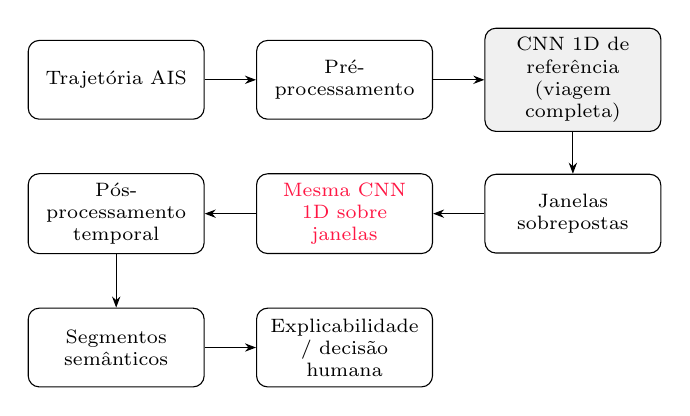
\begin{tikzpicture}[font=\scriptsize, >={Stealth[length=4pt]},
  box/.style={draw, rounded corners, align=center, minimum height=1.0cm, minimum width=2.2cm, text width=2.0cm},
  ref/.style={box, fill=gray!12}]
\node[box] (a) at (0,0) {Trajetória AIS};
\node[box] (b) at (2.9,0) {Pré-processamento};
\node[ref] (c) at (5.8,0) {CNN 1D de referência (viagem completa)};
\node[box] (d) at (5.8,-1.7) {Janelas sobrepostas};
\node[box] (e) at (2.9,-1.7) {\revtext{rev041}{Mesma CNN 1D sobre janelas}};
\node[box] (f) at (0,-1.7) {Pós-processamento temporal};
\node[box] (g) at (0,-3.4) {Segmentos semânticos};
\node[box] (h) at (2.9,-3.4) {Explicabilidade / decisão humana};
\draw[->] (a) -- (b);
\draw[->] (b) -- (c);
\draw[->] (c) -- (d);
\draw[->] (d) -- (e);
\draw[->] (e) -- (f);
\draw[->] (f) -- (g);
\draw[->] (g) -- (h);
\end{tikzpicture}
\captionof{figure}{Esquema do \emph{pipeline} proposto: a CNN 1D é usada primeiro sobre viagens completas (referência) e depois, \revtext{rev041}{a mesma rede,} sobre janelas com sobreposição.}
\label{fig:pipeline}
\end{center}

\subsection{\texorpdfstring{Pré-processamento e características}{Pré-processamento e características}}
\label{sec:abordagem-preproc}

Importação do CSV e recálculo, por viagem, dos intervalos temporais, distâncias, rumos, variações de rumo e velocidades a partir de $x$, $y$ e $t$, sem remoção de anomalias; seleção das características (velocidade, variação de rumo, intervalo temporal e distância à costa).

\subsection{\texorpdfstring{CNN de referência}{CNN de referência}}
\label{sec:abordagem-cnn-completa}

O modelo de referência é uma CNN 1D totalmente convolucional que recebe uma sequência de pontos e devolve uma probabilidade de pesca por ponto. É a \emph{mesma} rede nas duas experiências do trabalho: primeiro sobre a viagem completa, que é a referência propriamente dita e está fechada, e depois sobre janelas com sobreposição (Subsecção~\ref{sec:abordagem-janelas}). Manter a rede igual é o que permite atribuir qualquer diferença de desempenho ao janelamento e à sobreposição, e não a uma mudança do modelo.

Escolheu-se uma CNN pequena e simples como referência por três razões de desenho, que não são evidência: devolve naturalmente uma previsão por ponto, que é o que a segmentação exige; é leve (\resModParametros{} parâmetros), o que permite treinar e iterar só com CPU; e o seu contexto é local e conhecido (campo recetivo de \resModCampo{} pontos), o que facilita perceber o que o janelamento acrescenta ou não. A arquitetura é a proposta inicial do projeto, adotada como ponto de partida e não otimizada.

A entrada tem sete canais (quatro características normalizadas e três indicadores de ausência), e a normalização é ajustada apenas com as viagens de treino. Na viagem completa, cada viagem é uma sequência única, sem janelas, sem truncar e sem preenchimento de comprimento, com uma viagem por passo de treino. A especificação da rede, da perda e do treino está na Secção~\ref{sec:cnn-especificacao}, e os resultados da referência sobre a viagem completa na Secção~\ref{sec:resultados}.

\subsection{\texorpdfstring{Verificação da implementação}{Verificação da implementação}}
\label{sec:abordagem-verificacao}

O código desta fase foi verificado com testes automáticos sobre dados sintéticos e, para a leitura e a construção das sequências, sobre três viagens do conjunto de treino. Os testes confirmam: o alinhamento de cada previsão com o ponto e o instante de origem; que nenhum ponto passa de uma viagem para outra; o padrão esperado de valores em falta e das máscaras; a ausência de vazamento da monitorização interna para a normalização; a rejeição de ficheiros e identificadores de validação e teste; as dimensões da saída para comprimentos diferentes; o campo recetivo de \rv{\resModCampo} pontos; e que a perda, os gradientes e um passo do otimizador funcionam. Estes testes verificam o código e não medem a qualidade do modelo. \revtext{rev040}{Os resultados estão na Subsecção~\ref{sec:cnn-treino}; o conjunto de teste serviu apenas para escolher a época e o limiar, e o de validação não foi aberto.}

\subsection{\texorpdfstring{\revtext{rev023}{Janelamento com sobreposição}}{Janelamento com sobreposição}}
\label{sec:abordagem-janelas}

\revtext{rev041}{A mesma CNN de referência (Secção~\ref{sec:cnn-especificacao}), sem alterações à arquitetura, é treinada e avaliada sobre janelas de comprimento fixo $L$ com sobreposição, para medir se o janelamento e a sobreposição melhoram a segmentação face à viagem completa. Começa-se com $L=64$ pontos e com sobreposição de 0\,\% (controlo, que separa o efeito do janelamento do efeito da sobreposição) e de 50\,\%; depois testa-se se aumentar ou diminuir $L$ compensa. Cada janela devolve uma probabilidade por ponto, e cada ponto original recebe a média das probabilidades das janelas em que aparece; a avaliação conta uma previsão por ponto original, e o preenchimento da última janela é ignorado na perda, na média e nas métricas. A divisão dos dados, as características, o normalizador e as métricas mantêm-se, para que a única diferença seja o janelamento. Ficam por decidir se a sobreposição se aplica no treino, na inferência ou em ambos, e o orçamento de treino, porque a mesma quantidade de épocas não dá o mesmo número de passos. Esta fase ainda não foi implementada.}

\subsection{\texorpdfstring{\revtext{rev023}{Pós-processamento temporal}}{Pós-processamento temporal}}
\label{sec:abordagem-pos}

\revtext{rev021}{As probabilidades por ponto são suavizadas (por exemplo, por votação por vizinhança\revtext{rev042}{, com a unidade e a largura por definir}), produzindo segmentos contíguos e estáveis.}

\subsection{\texorpdfstring{\revtext{rev023}{Saída, explicabilidade e ferramentas}}{Saída, explicabilidade e ferramentas}}
\label{sec:abordagem-saida}

\revtext{rev021}{Trajetória segmentada com confiança por segmento e justificações (importâncias de características) que apoiam --- e não substituem --- o inspetor. A divisão dos dados e as características são as mesmas em todas as fases, para que as comparações sejam diretas.} A implementação usa Python, PyTorch, scikit-learn e pandas.

\section{\texorpdfstring{Especificação da CNN 1D de referência}{Especificação da CNN 1D de referência}}
\label{sec:cnn-especificacao}

Esta secção descreve a rede com o detalhe necessário para a recriar com os mesmos valores. Indica-se também, para cada escolha, o motivo e o seu estado: o que foi \emph{decidido}, o que foi \emph{adotado como valor inicial} sem validação, e o que \emph{ainda não está definido}. Nenhum valor desta secção foi otimizado com os dados: a arquitetura é a proposta inicial do protocolo do projeto, declarada ``por validar''. \revtext{rev041}{A especificação vale para as duas experiências, a viagem completa e as janelas. Os resultados estão na Secção~\ref{sec:resultados}.}

\subsection{\texorpdfstring{Entrada e saída}{Entrada e saída}}

A rede processa \revtext{rev041}{uma sequência de cada vez: a viagem completa ou, na experiência com janelamento, uma janela.} A entrada é uma matriz $X\in\mathbf{R}^{7\times N}$, em que $N$ é o número de pontos da \revtext{rev041}{sequência (varia de viagem para viagem; numa janela é o comprimento fixo $L$)} e as sete linhas, por esta ordem, são: velocidade (\texttt{speed\_calc\_mps}), variação de rumo com sinal (\texttt{signed\_turn\_calc\_deg}), intervalo temporal (\texttt{time\_gap\_calc\_s}), distância à costa (\texttt{distanceToShore}), e os indicadores de ausência da velocidade, da variação de rumo e do intervalo temporal (1 se o valor original faltava, 0 caso contrário). As quatro primeiras linhas são normalizadas com a média e o desvio-padrão populacional de cada característica, calculados só com as viagens de treino e ignorando valores em falta; depois de normalizar, os valores em falta ficam a zero (a média). Os identificadores, os instantes, $x$ e $y$ não são entradas. A saída é um vetor de $N$ \emph{logits}, um por ponto original, $z\in\mathbf{R}^{N}$; a probabilidade de pesca é $p_i=\sigma(z_i)=1/(1+e^{-z_i})$, calculada só na inferência. \revtext{rev041}{Na viagem completa não há janelas, truncagem nem preenchimento de comprimento, e o lote tem sempre uma só viagem; com janelas, o preenchimento da última janela é marcado e ignorado na perda.}

\subsection{\texorpdfstring{Arquitetura}{Arquitetura}}

A rede é totalmente convolucional e está resumida na Tabela~\ref{tab:cnn-arquitetura}. Todas as convoluções têm \emph{stride} 1, dilatação 1 e \emph{padding} de zeros de $\lfloor k/2\rfloor$ posições em cada extremo, de modo que o comprimento $N$ se mantém. Não existem camadas de \emph{pooling}, normalização de lote, \emph{dropout} nem sigmoide. O número de parâmetros de uma convolução é $C_\text{in}\,C_\text{out}\,k+C_\text{out}$; o total é \rv{\resModParametros}, obtido por contagem no código. A Figura~\ref{fig:cnn-desenho} mostra o desenho da rede e o campo recetivo.

\begin{table}[t]
\centering\small
\begin{tabular}{@{}llrr@{}}
\toprule
Camada & Canais (entrada$\to$saída) & $k$ & Parâm. \\
\midrule
Conv1D + ReLU & $7\to32$  & 5 & \rv{\resModParamA} \\
Conv1D + ReLU & $32\to64$ & 5 & \rv{\resModParamB} \\
Conv1D + ReLU & $64\to32$ & 5 & \rv{\resModParamC} \\
Conv1D (cabeça) & $32\to1$  & 1 & \rv{\resModParamD} \\
\midrule
Total & & & \rv{\resModParametros} \\
\bottomrule
\end{tabular}
\caption{Arquitetura da CNN 1D de referência. A saída são \emph{logits} de forma $1\times N$.}
\label{tab:cnn-arquitetura}
\end{table}

\begin{figure*}[t]
\centering
\resizebox{\textwidth}{!}{%
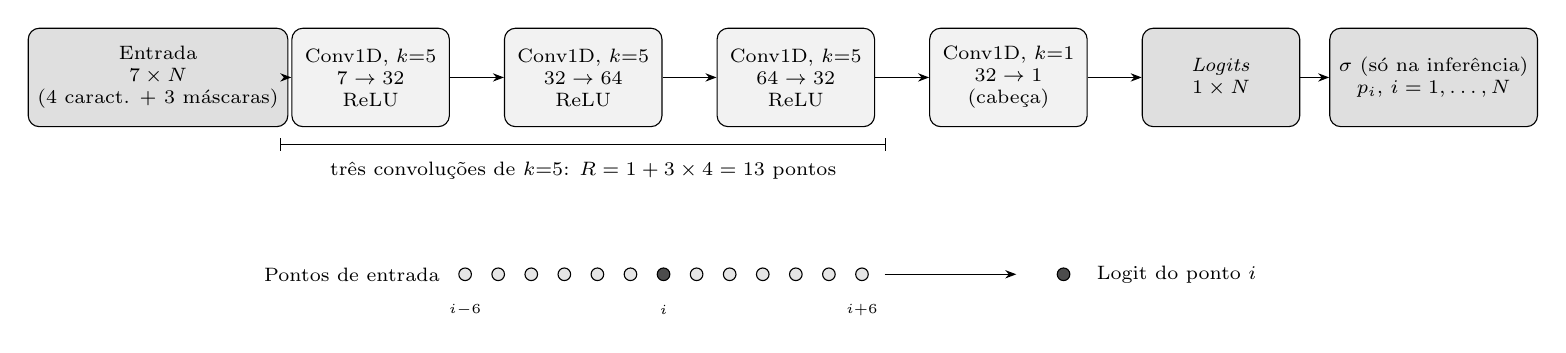
\begin{tikzpicture}[font=\scriptsize, >={Stealth[length=4pt]},
  blk/.style={draw, rounded corners, align=center, minimum height=1.25cm, minimum width=2.0cm, fill=gray!10},
  io/.style={draw, rounded corners, align=center, minimum height=1.25cm, minimum width=2.0cm, fill=gray!25},
  pt/.style={circle, draw, inner sep=0pt, minimum size=0.16cm, fill=gray!20},
  sel/.style={circle, draw, inner sep=0pt, minimum size=0.16cm, fill=black!70}]
% cadeia principal
\node[io]  (in) at (0,0)    {Entrada\\$7\times N$\\(4 caract. + 3 máscaras)};
\node[blk] (c1) at (2.7,0)  {Conv1D, $k{=}5$\\$7\to32$\\ReLU};
\node[blk] (c2) at (5.4,0)  {Conv1D, $k{=}5$\\$32\to64$\\ReLU};
\node[blk] (c3) at (8.1,0)  {Conv1D, $k{=}5$\\$64\to32$\\ReLU};
\node[blk] (c4) at (10.8,0) {Conv1D, $k{=}1$\\$32\to1$\\(cabeça)};
\node[io]  (z)  at (13.5,0) {\emph{Logits}\\$1\times N$};
\node[io]  (p)  at (16.2,0) {$\sigma$ (só na inferência)\\$p_i$, $i=1,\dots,N$};
\foreach \a/\b in {in/c1,c1/c2,c2/c3,c3/c4,c4/z,z/p}{\draw[->] (\a) -- (\b);}
% chaveta do campo recetivo
\draw[Bar-Bar] (1.55,-0.85) -- (9.25,-0.85)
  node[midway,below=3pt]{três convoluções de $k{=}5$: $R=1+3\times4=13$ pontos};
% esquema do campo recetivo
\foreach \j in {-6,...,6}{
  \pgfmathsetmacro{\xx}{3.9+0.42*(\j+6)}
  \ifnum\j=0 \node[sel] (e\j) at (\xx,-2.5) {};\else\node[pt] (e\j) at (\xx,-2.5) {};\fi}
\node[sel] (o) at (11.5,-2.5) {};
\draw[->] (e6.east) ++(0.2,0) -- (10.9,-2.5);
\node[anchor=east] at (3.7,-2.5) {Pontos de entrada};
\node[anchor=west] at (11.8,-2.5) {Logit do ponto $i$};
\node[font=\tiny] at (3.9,-2.95) {$i{-}6$};
\node[font=\tiny] at (6.42,-2.95) {$i$};
\node[font=\tiny] at (8.94,-2.95) {$i{+}6$};
\end{tikzpicture}}
\caption{Desenho da CNN 1D de referência. Em cima, a cadeia de camadas: \revtext{rev041}{uma sequência de $N$ pontos (a viagem inteira ou uma janela), com 7 canais,} passa por três Conv1D com \emph{kernel} 5 (32, 64 e 32 filtros, ReLU) e por uma cabeça de \emph{kernel} 1, que devolve um \emph{logit} por ponto; a sigmoide só se aplica na inferência. O comprimento $N$ mantém-se em todas as camadas. Em baixo, o campo recetivo: cada saída depende dos \rv{\resModCampo} pontos de entrada entre $i-6$ e $i+6$.}
\label{fig:cnn-desenho}
\end{figure*}

\subsection{\texorpdfstring{Porquê estes valores}{Porquê estes valores}}

\textbf{Número de camadas e filtros (32, 64, 32).} Estes valores \emph{não} resultam de uma pesquisa nem de experiências: são os da arquitetura ilustrativa do protocolo do projeto, adotados como ponto de partida e declarados por validar. O raciocínio que os suporta é de desenho, não uma evidência: três camadas convolucionais dão à rede capacidade para combinar velocidade, curvatura, intervalo e distância à costa em padrões locais de movimento, e a forma ``alargar e voltar a estreitar'' (32, 64, 32) cria uma representação intermédia mais rica antes de a cabeça a resumir num único \emph{logit}. A rede é pequena (\rv{\resModParametros} parâmetros) de propósito: o equipamento disponível tem apenas CPU e 16~GB de memória, e um modelo pequeno permite iterar sem GPU. Se este tamanho é suficiente ou excessivo para este problema, não se sabe; só uma comparação com outras larguras ou profundidades, que não faz parte do âmbito atual, o poderia dizer.

\textbf{\emph{Kernel} 5.} Um \emph{kernel} ímpar permite um \emph{padding} simétrico que preserva o comprimento sem deslocar a previsão em relação ao ponto. O valor 5 é o da arquitetura inicial do protocolo; com três camadas determina o campo recetivo de \rv{\resModCampo} pontos (abaixo). É um valor adotado, não ajustado. Note-se que o campo recetivo é medido em \emph{pontos} e não em tempo: como o intervalo entre pontos varia, \rv{\resModCampo} pontos não correspondem a uma duração fixa.

\textbf{Cabeça com \emph{kernel} 1.} A última camada combina, em cada ponto, os 32 canais num só \emph{logit}, sem olhar para pontos vizinhos. Assim, todo o contexto temporal vem das três camadas anteriores e a cabeça não aumenta o campo recetivo. Um \emph{kernel} 1 devolve um valor por ponto, como exigido; uma camada final que reduzisse a viagem a um só valor seria incompatível com uma previsão por ponto.

\textbf{ReLU, sem normalização de lote nem \emph{dropout}.} A ReLU é a ativação padrão em CNN, simples e sem parâmetros. Não se acrescentaram normalização de lote nem \emph{dropout} para manter a rede mínima e não introduzir mais hiperparâmetros antes de existir uma referência; não foi testado se ajudariam.

\subsection{\texorpdfstring{Campo recetivo}{Campo recetivo}}

O campo recetivo é o número de pontos de entrada que influenciam uma saída. Com \emph{stride} 1 e dilatação 1, cada convolução de \emph{kernel} $k$ acrescenta $k-1$ pontos, pelo que
\begin{equation}
R = 1+\sum_{i}(k_i-1) = 1+3\times4+0 = 13 .
\end{equation}
Isto significa que a previsão para o ponto $i$ depende dos pontos $i-6,\dots,i+6$ e de mais nenhum. Está verificado por teste: perturbar a entrada num ponto altera as saídas apenas nesses \rv{\resModCampo} pontos. Consequência importante: \emph{entrada completa não significa contexto global}. Embora a viagem inteira entre na rede, cada previsão usa uma vizinhança curta; comportamentos longos (por exemplo, um percurso de pesca com horas de duração) só são vistos através de vizinhanças locais. Nos primeiros e últimos seis pontos, o \emph{padding} de zeros faz a rede ver ``pontos fictícios'' com todas as características e indicadores a zero, o que, no espaço normalizado, equivale a valores médios sem ausência; é uma escolha por omissão da biblioteca, cujo efeito nas fronteiras não foi estudado.

\subsection{\texorpdfstring{Função de perda}{Função de perda}}

A perda é a entropia cruzada binária aplicada aos \emph{logits}, com média sobre os pontos da \revtext{rev041}{sequência (uma viagem ou uma janela)}:
\begin{equation}
\mathcal{L}=-\frac1N\sum_{i=1}^{N}\Big[y_i\log\sigma(z_i)+(1-y_i)\log\big(1-\sigma(z_i)\big)\Big],
\end{equation}
com $y_i=1$ para pesca e $0$ para navegação. Usa-se a versão que recebe \emph{logits} (\texttt{BCEWithLogitsLoss}), que combina a sigmoide e o logaritmo numa forma numericamente estável; por isso a rede não tem sigmoide na saída e esta não é aplicada duas vezes. Todos os pontos entram na perda, incluindo os pontos iniciais com valores em falta, que têm máscara na entrada. Não se usam pesos de classe nem reamostragem, por decisão do projeto: o desequilíbrio natural entre pesca e navegação é mantido e pode enviesar o modelo para a classe maioritária; é uma limitação a observar nos resultados. Como cada passo de treino usa uma só viagem e a perda é a média dessa viagem, cada viagem pesa o mesmo \emph{por passo}, independentemente do comprimento; viagens longas têm assim, por ponto, menos peso do que viagens curtas.

\subsection{\texorpdfstring{Otimizador e treino}{Otimizador e treino}}

O otimizador previsto é o Adam, que adapta o passo de cada parâmetro e costuma funcionar sem grande ajuste, o que o torna uma escolha razoável para uma referência. Está implementado sem decaimento de pesos nem calendário de taxa de aprendizagem. A taxa de aprendizagem $10^{-3}$ no código é apenas o valor por omissão do Adam, usado como \emph{marcador}: \textbf{não foi escolhida nem validada} e será fixada na configuração de execução. Os restantes parâmetros foram fixados na configuração do treino (Subsecção~\ref{sec:cnn-treino}) e são igualmente iniciais e não validados. Cada passo de otimização usa uma viagem completa (\emph{batch} de tamanho 1), em ordem aleatória reprodutível. \revtext{rev041}{Na experiência com janelas, o tamanho do lote e o orçamento de treino ainda estão por definir.}

\subsection{\texorpdfstring{Reprodutibilidade}{Reprodutibilidade}}

Os pesos iniciais são os da inicialização por omissão do PyTorch (\rv{\resTrTorch}, CPU) para camadas convolucionais, e a semente do gerador (Python, NumPy e PyTorch) é fixada na execução; a semente da divisão dos dados é 42. A ordem de treino das viagens usa um gerador com semente própria. O código regista a semente, as versões e o número de \emph{threads}, mas não garante resultados idênticos entre máquinas diferentes.  A configuração do treino (semente \resTrSemente{} e os valores acima) está no ficheiro \texttt{configs/phase1\_select.json}. Cada execução grava a semente, as versões, o normalizador e os hashes dos ficheiros usados. A escolha da época e do limiar segue um protocolo declarado antes de abrir o conjunto de teste e fica registada, e todos os números desta secção vêm do ficheiro \texttt{results/baseline\_frozen/final\_results.json}, gerado por \texttt{build\_final\_results.py}.

\section{Materiais e Dados}
\label{sec:materiais-dados}

Será usado o conjunto público \emph{Detailed Labelled Fishing Trajectories from AIS} (Kaggle)~\cite{kaggleAIS}: \rv{\resDadosViagens} trajetórias de pesca anotadas, com \rv{\resDadosLinhas} pontos (linhas), 13 colunas --- 12 atributos (identificador do navio e da viagem, instante, longitude, latitude, coordenadas projetadas, rumo, distância à costa, entre outros) e um rótulo. As cinco classes, desequilibradas (pesca: \texttt{02-fishing}, \texttt{04-fishing}; navegação: \texttt{01-sailing}, \texttt{03-sailing}, \texttt{05-sailing}), são agregadas num problema binário, mantendo o desequilíbrio natural (sem reamostragem nem pesos de classe) e as trajetórias completas.

Eticamente, apesar de públicos, os dados AIS usados em fiscalização exigem cuidado: a deteção automática não deve, por si só, fundamentar sanções (a decisão humana é obrigatória); o sistema deve ser transparente e justo, evitando enviesamentos contra tipos de navio, regiões ou comunidades de pesca; e a confiança deve ser calibrada para não induzir falsa segurança.

\subsection{Tratamento dos dados}
\label{sec:tratamento-dados}

Os dados são usados tal como existem, sem remoção de linhas. As anomalias (saltos de posição, \emph{gaps} temporais longos e inversões de rumo) são mantidas, porque o sistema visa dados AIS ao momento, onde estes erros ocorrem; removê-las na preparação tornaria a avaliação otimista, e a robustez a estas anomalias faz parte do que se avalia. Uma função de preparação recalcula, por viagem (mesmo identificador), as grandezas derivadas a partir das bases $x$, $y$, $t$ e distância à costa: intervalo temporal (\texttt{time\_gap}, em segundos), distância entre pontos consecutivos (\texttt{distance\_gap}, em metros), rumo (\texttt{bearing}, em graus, medido a partir do eixo $y$ da grelha UTM), variação de rumo com sinal (\texttt{signed\_turn}, em graus, no intervalo (-180, 180]) e velocidade (em nós). O rótulo binário (\texttt{target}) resulta do mapeamento das cinco classes em pesca e navegação. O primeiro ponto de cada viagem não tem anterior e fica com valores ausentes nas grandezas que dependem dele. Os valores recalculados coincidem com os originais do conjunto em \rv{\resPrepCoincide} dos pares (no mínimo, entre as três grandezas comparadas). O rumo da grelha difere do rumo em norte verdadeiro em \rv{\resPrepBearingMediana}\textdegree{} (mediana), pela convergência dos meridianos. A distância à costa é usada tal como vem no conjunto, sem verificação externa. A preparação aplica-se a cada conjunto separadamente, a partir do manifesto de divisão, e é verificada com testes sintéticos.

Na CNN, o primeiro ponto de cada viagem não tem \texttt{time\_gap}, \texttt{speed} nem \texttt{signed\_turn}, e o segundo não tem \texttt{signed\_turn}. Esses valores em falta são preenchidos com zero e marcados por um indicador de ausência, para distinguir ausência de valor zero. Estes pontos entram na função de perda. Nenhuma linha é removida.

\section{Avaliação}
\label{sec:avaliacao}

\subsection{\texorpdfstring{\revtext{rev023}{Métricas e estudo de ablação}}{Métricas e estudo de ablação}}
\label{sec:avaliacao-metricas}

Quantitativamente, medem-se precisão, sensibilidade, F1 e IoU por segmento (e por ponto), \revtext{rev042}{comparando a CNN sobre janelas com a CNN de referência sobre a viagem completa}. Um estudo de ablação com quatro variantes isola cada componente: (i) sem sobreposição nem pós-processamento; (ii) só sobreposição; (iii) só pós-processamento; (iv) ambos (método proposto). Analisa-se também a robustez face à taxa de sobreposição (0\%, 25\%, 50\%, 75\%) e ao nível de regularização temporal. A estabilidade mede-se pela fragmentação (número de segmentos por trajetória) e pelo erro de fronteira (desvio entre início/fim previsto e real); ``estável'' designa uma segmentação que muda pouco sob pequenas alterações da janela ou do pós-processamento.

\subsection{\texorpdfstring{Divisão dos dados e protocolo}{Divisão dos dados e protocolo}}
\label{sec:avaliacao-protocolo}

Os dados são divididos por trajetória completa (ID completo, composto pelo identificador do navio e pelo sufixo da viagem) em treino, validação e teste, na proporção 70/15/15, com semente 42 e manifesto fixo. Todas as linhas de cada trajetória ficam no mesmo conjunto. Trajetórias do mesmo navio podem pertencer a conjuntos diferentes, por decisão do projeto; por isso, os resultados não são apresentados como generalização para navios inéditos. Os hiperparâmetros e as restantes escolhas (número de épocas, limiar, variantes) usam apenas o treino e o conjunto de teste, que serve para selecionar; o conjunto de validação é reservado à medição final, feita uma só vez com o modelo e o protocolo congelados.

\subsection{\texorpdfstring{\revtext{rev023}{Avaliação qualitativa e dimensão humana}}{Avaliação qualitativa e dimensão humana}}
\label{sec:avaliacao-qualitativa}

Qualitativamente, produzir-se-ão mapas das trajetórias com os segmentos preditos sobrepostos à verdade de referência e analisar-se-ão casos de sucesso e falha. Para a dimensão HCAI~\cite{shneiderman2020}, prevê-se avaliar de forma preliminar a explicabilidade (verificando se as atribuições~\cite{lundberg2017} correspondem aos padrões de movimento esperados) e a utilidade como apoio à decisão, através de um \emph{dashboard} de prova de conceito com segmentação, confiança calibrada~\cite{guo2017} e justificações.

\section{\texorpdfstring{\revtext{rev041}{Resultados}}{Resultados}}
\label{sec:resultados}

\revtext{rev041}{Esta secção reúne os resultados da CNN de referência: sobre a viagem completa (Subsecção~\ref{sec:cnn-treino}) e, depois, com janelamento (Subsecção~\ref{sec:resultados-janelas}). A rede é a mesma em todos os casos, para que as diferenças se devam só ao janelamento e à sobreposição.}

\subsection{\texorpdfstring{CNN de referência sobre a viagem completa}{CNN de referência sobre a viagem completa}}
\label{sec:cnn-treino}

Esta é a CNN de referência sobre a viagem completa, e está fechada: o modelo, a época e o limiar não voltam a mudar, e os valores abaixo são o termo de comparação com a CNN com janelamento.

O treino usou todo o conjunto de treino oficial (\resTrViagens{} viagens, \resTrPontos{} pontos), sem monitorização interna: o normalizador foi ajustado com essas viagens e todas serviram para ajustar a rede. Usou-se o Adam (taxa de aprendizagem $10^{-3}$) durante \resTrEpocas{} épocas, sem paragem antecipada, com a semente \resTrSemente{}, e guardou-se um modelo no fim de cada época. O treino durou cerca de \resTrSegundos{} minutos num CPU (cerca de \resTrSegPorEpoca{} segundos por época). Estes valores são iniciais e não foram validados.

A época e o limiar de classificação foram escolhidos no conjunto de teste (\resSelViagens{} viagens, \resSelPontos{} pontos), numa única ronda e com critérios declarados antes de o abrir: a época com a menor perda por ponto entre as \resSelNCand{} candidatas e, nessa época, o limiar entre \resSelGrelhaMin{} e \resSelGrelhaMax{} (passo 0,05) que maximiza a média dos F1 das duas classes. Resultaram a época \resSelEpoca{} e o limiar \resSelLimiar{}, e o modelo ficou congelado. O conjunto de validação não foi aberto e fica reservado à medição final, que será feita uma só vez no fim do trabalho.

A Tabela~\ref{tab:resultados} e a Figura~\ref{fig:final-matriz} mostram o desempenho por ponto do modelo congelado nas viagens de treino e nas de teste. Os do treino medem o ajuste; os do teste são \textbf{otimistas}, porque esse conjunto serviu para escolher a época e o limiar, e não substituem a medição final no conjunto de validação. No teste, a exatidão foi \resTesteAcc{} (\resTesteErros{} erros em \resTestePontos{} pontos), contra \resTesteAccMaj{} de uma regra que prevê sempre a classe maioritária (pesca, \resTestePercPesca{} dos pontos do teste); no treino foi \resTreinoAcc{}, contra \resTreinoAccMaj{}. Por viagem de teste (Figura~\ref{fig:final-viagens}), a exatidão vai de \resTesteViagMin{} (viagem \resTestePiorViagem) a \resTesteViagMax{}, com mediana de \resTesteViagMed{}; o número de viagens de teste em que a CNN não supera a regra da classe maioritária dessa viagem é \resTesteNViagNaoSuperam{}.

A perda por ponto no teste oscila muito de época para época (Figura~\ref{fig:final-perda}): na época escolhida vale \resSelPerdaTeste{}, mas desde a época 100 chega a \resSelPerdaTesteMax{}, enquanto no treino vale \resSelPerdaTreino{} na mesma época e varia menos. A escolha da época é, por isso, sensível a essa oscilação, e o conjunto de teste tem só \resSelViagens{} viagens.

\begin{table}[t]
\centering\footnotesize
\begin{tabular}{@{}llrrrrr@{}}
\toprule
Conjunto & Classe & Pontos & Prec. & Sensib. & F1 & IoU \\
\midrule
Treino & Navegação & \resTreinoNavReal & \resTreinoNavPrec & \resTreinoNavSens & \resTreinoNavF & \resTreinoNavIoU \\
Treino & Pesca & \resTreinoPescaReal & \resTreinoPescaPrec & \resTreinoPescaSens & \resTreinoPescaF & \resTreinoPescaIoU \\
Teste & Navegação & \resTesteNavReal & \resTesteNavPrec & \resTesteNavSens & \resTesteNavF & \resTesteNavIoU \\
Teste & Pesca & \resTestePescaReal & \resTestePescaPrec & \resTestePescaSens & \resTestePescaF & \resTestePescaIoU \\
\bottomrule
\end{tabular}
\caption{Métricas por ponto e por classe do modelo congelado (época \resSelEpoca{}, limiar \resSelLimiar{}). ``Pontos'' são os pontos reais de cada classe. Os resultados do teste são otimistas (esse conjunto serviu para escolher).}
\label{tab:resultados}
\end{table}

\begin{figure}[t]
\centering
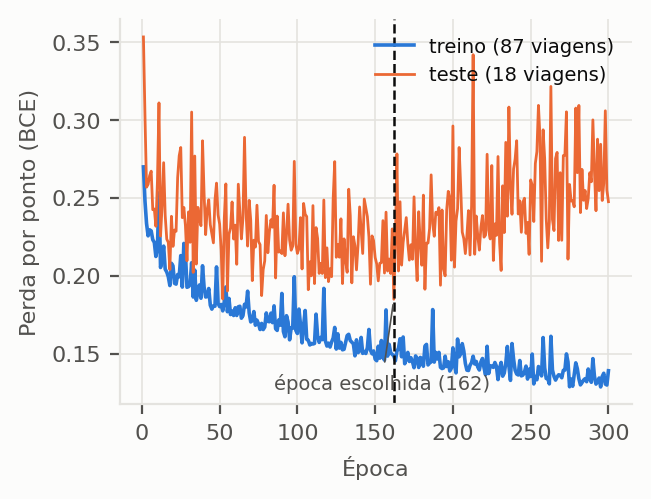
\includegraphics[width=0.95\columnwidth]{figures/final_perda.png}
\caption{Perda por ponto (entropia cruzada binária) ao longo das épocas, avaliada no fim de cada época nas viagens de treino e nas de teste. A linha tracejada marca a época escolhida no teste.}
\label{fig:final-perda}
\end{figure}

\begin{figure}[t]
\centering
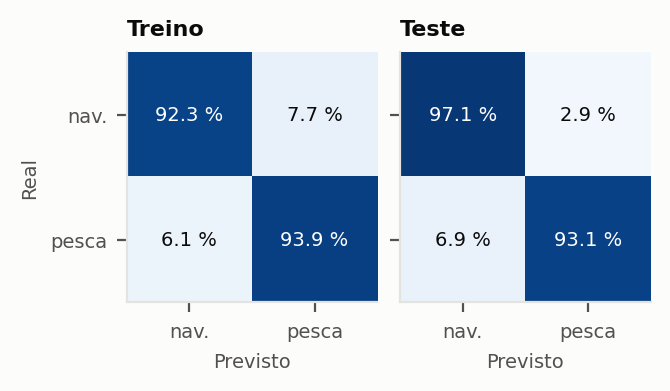
\includegraphics[width=0.95\columnwidth]{figures/final_matriz.png}
\caption{Matrizes de confusão por ponto do modelo congelado: percentagem da classe real (linha) prevista em cada classe, nas viagens de treino e nas de teste.}
\label{fig:final-matriz}
\end{figure}

\begin{figure*}[t]
\centering
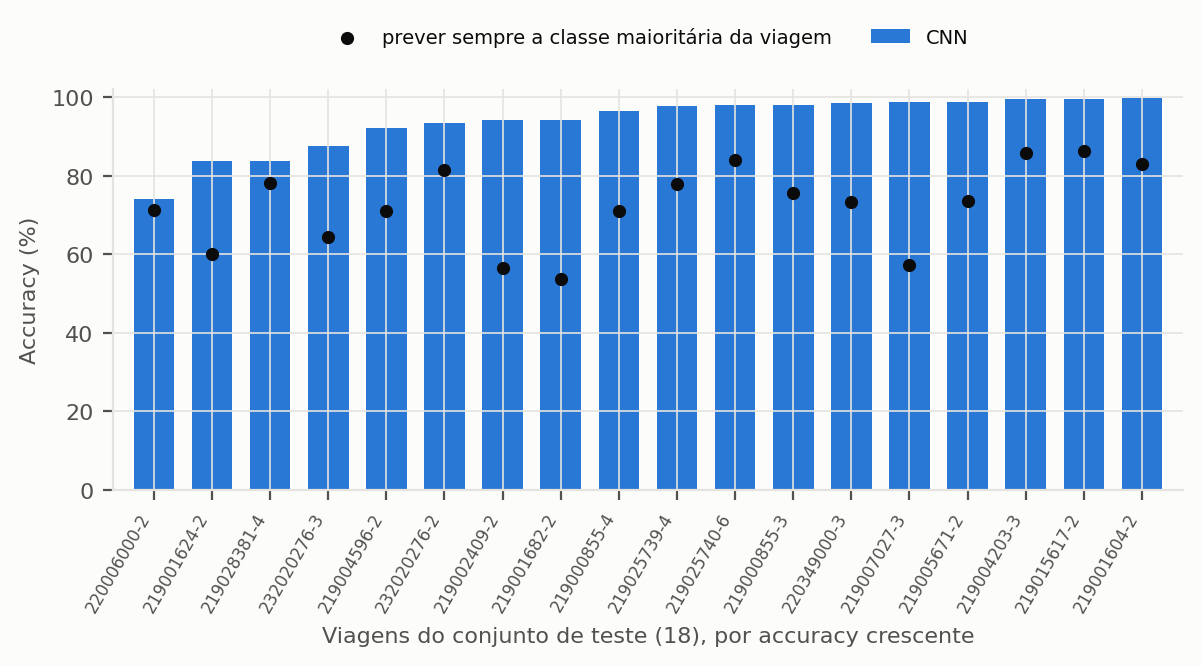
\includegraphics[width=0.82\textwidth]{figures/final_viagens.png}
\caption{Exatidão por viagem do conjunto de teste (barras, por ordem crescente) e exatidão de uma regra que prevê sempre a classe maioritária dessa viagem (pontos).}
\label{fig:final-viagens}
\end{figure*}

\subsection{\texorpdfstring{\revtext{rev041}{CNN de referência com janelamento}}{CNN de referência com janelamento}}
\label{sec:resultados-janelas}

\revtext{rev041}{Ainda não foram feitos. Quando existirem, esta subsecção apresenta os resultados da mesma CNN de referência sobre janelas de $L=64$ pontos, com sobreposição de 0\,\% e de 50\,\%, comparados com os da subsecção anterior com as mesmas métricas e a mesma divisão, e depois o efeito de aumentar ou diminuir $L$. É esta comparação com a viagem completa que responde à RQ1 (Secção~\ref{sec:objetivos}).}

% References may use the provided IJCAI named bibliography style.
\bibliographystyle{FormattingGuidelines-IJCAI-ECAI-26/named}
\bibliography{references}

\end{document}
